\synctex=1

\documentclass[11pt]{article}
\usepackage[margin=1.2in,letterpaper]{geometry}
\usepackage{amssymb}
\usepackage{hyperref}
%\usepackage[tiny,compact]{titlesec}
\usepackage{graphicx}
\usepackage{todo}
\usepackage{booktabs}
	\usepackage{multirow}
\usepackage{afterpage}
\usepackage{verbatim}
\usepackage{array}
\usepackage{multirow}
\usepackage{framed}
\usepackage{hanging}
%\usepackage{supertabular}
\usepackage{mathtools}
\usepackage[all]{xy}
\usepackage{ot-tableau}
\usepackage{hanging}
\usepackage{paralist} 
\usepackage{caption}
\usepackage{subcaption}
\usepackage{fancyhdr} 
\usepackage{sectsty}
%\allsectionsfont{\sffamily\mdseries\upshape} 
\usepackage{float}
\usepackage[nottoc,notlof,notlot]{tocbibind} 
\usepackage[titles,subfigure]{tocloft} 



%\usepackage[explicit]{titlesec}
%\usepackage{type1cm}
%\usepackage{xcolor}

\usepackage{xltxtra} % Loads fontspec, xunicode, metalogo, fxltx2e, and some extra customizations for XeLaTeX
\defaultfontfeatures{Mapping=tex-text} % to support TeX conventions like ``---''
\setmainfont{Charis SIL}

\usepackage[sort]{natbib}
\bibpunct[:]{(}{)}{,}{a}{}{,}

\usepackage{gb4e} \let\eachwordone=\sl \let\eachwordthree=\sf

\newcommand{\mcom}[1]
{\mbox{}\marginpar{\raggedleft\raggedright\hspace{0pt}\footnotesize{#1}}}
\newcommand{\note}[1]{{ }\mcom{Note}\textbf{#1}}

\pagestyle{fancy}
\fancyhf{}
\rhead{\tiny JP\hspace{2cm}\textbf{\thepage}}
\rfoot{}

\renewcommand{\headrulewidth}{0pt} 


\title{\large Proposal\\\Large \textbf{Relative tense in Arnhem land}}
\date{\today}
\author{Josh}

\date{\today}


\begin{document}\thispagestyle{empty}
\part*{The Meaning, Development of Relative Tense in Yolŋu}
\begin{itemize}
\item 

Yolŋu Matha is a Pama-Nyungan dialect continuum spoken in northern Arnhem land on the Arafura coast of Northern Australia. It consists of six identified dialect groups. The dialects are mutually intelligible. Nevertheless, the semantics of their cognate tense suffixes exhibit some interesting variation.

\item There are four types of tense inflection. Of particular concern to us currently are what Wilkinson refers to as the FIRST (I) and THIRD (III) inflections (in other works dubbed \textit{contemporary and precontemporary.}) Her partial analysis, similar to Comrie's for Burarra (1985:89) suggests that these are exponents of relative tense. Comrie's Burarra data is summarised below for the verb \textit{ŋupa-} `eat':


\begin{tabular}{llll}
INFL$\backslash$FRAME && \textit{today} & $\neg$\textit{today}\\\midrule
CLOSE&\textit{ŋupaŋa}& I am eating & I ate within the past few days\\
REMOTE&\textit{ŋupade} & I ate today & I ate long ago
\end{tabular}


\item A similar pattern to that of Djamparrpuyŋu (Dhuwal dialect) described below occurs for Gupapuyŋu and Djinaŋ (Yolŋu) as well as Nakarra and Burarra ([non-PN] Arnhem). The Arnhem and Yolŋu families are unrelated.

\item The pattern does not hold for Eastern dialects of Yolŋu Matha: Djapu or Ritharrŋu. It is reasonable to infer that this `discontinuous' relative tense system is an areal feature.
\end{itemize}
\begin{framed}
\vspace{-.4cm}\section*{Some thoughts on tense}
Tense is largely modelled as a \underline{deictic system}.\\\begin{tabular}{ll}
\textit{person} & {\sc speaker/hearer}\\
\textit{time} & {\sc now}\\
\textit{location} & {\sc here}
\end{tabular}


\vspace{.5cm}
``What's crucial to all tense specifications, however is the need for a deictic centre, or reference point... so far we have assumed that the deictic centre for tense will be a single point in time.  \textbf{The question therefore arises whether all tenses can be described in terms of such deictic centres}.'' (Comrie 1985: 17)

\vspace{.5cm}
Finite verb forms in English are taken to always encode `absolute time reference'. `[N]on-finite forms characteristically have relative time reference' (\textit{cf. also time adverbials)}
\begin{exe}\ex
\textit{the people sitting on the bench were arrested}\ex \textit{the passengers denied boarding to QF4 proceeded to gate 27}\end{exe}


\vspace{.5cm}
`\textbf{metrical}' tense systems `...provide an approximate and subjective measure of the interval between the frame and the tense locus' (Chung \& Timberlake 1985: 207)
 \vspace{0.5cm}
 
 `\textbf{cyclical}' tense systems: `two oppostions... absolute cut-off point between today and earlier than today, the other between recent and remote within each of these two time frames' (Comrie 1985: 89).\end{framed}
\section*{The phenomenon}

\subsection*{Djambarrpuyŋu (Western Yolŋu)}
\textbf{Djambarrpuyŋu} (Yolŋu): `use of two inflections: one to code realized events closest to the speaker's moment of speech (the Contemporary tenses --- present;yesterday/recent) and another to code Pre-contemprary events (earlier today and remote past)' (Wilkinson 1991: 339).
\begin{exe}\ex\begin{xlist}
\ex\gll gunga mala ga dhaarra'-dharra\\
pandanus tree {\sc ipfv} stand$\sim${\sc redup}\textbf{.I}\\
\glt`The pandanus trees are standing (there)'
\ex\gll nhaakurr nhuma ga ŋirrimbu-m\\
where 2.nsg {\sc ipfv} go\textbf{-I}\\
`where are you going?'\end{xlist}
\ex\begin{xlist}\ex\gll yo barpuruɲ ŋarra ŋaɲa nhaa-\textbf{ma}-ɲ (*nhaaŋal)\\
yes, yesterday{\sc-prom} 1s 3s{\sc.acc} see-\textbf{I}-{\sc prom}\\
\glt`Yes, I saw him yesterday'
\ex\gll ŋe gaathur ŋarra ŋaɲa nhaa-\textbf{ŋal} goḍarr dhiyal\\
yes, today 1s 3s{\sc.acc} see-\textbf{III} morning {\sc prox-loc}\\
\glt`Yes, I saw him here this morning'
\ex\gll maarrma ga-\textbf{n} malwan-dja dhaara-\textbf{n} yindi maṉḍa-ɲ\\
two {\sc ipfv-\textbf{III}} Hibiscus-{\sc prom} stand-\textbf{III} big 3d-{\sc prom}\\
\glt`Two big Hibiscus flowers were growing there' (at some place in the speaker's youth)
\end{xlist}\end{exe}
\footnotesize
Frequently cooccur with adverbials: \begin{description}
\item[ŋaathil] `prior/before' (remote past)
\item[barpuru] `yesterday' (recent past)
\item[yawuŋu] `recently' (recent past)
\item[gaathur] `these days' (today past, present, today future [with \textit{dhu} {\sc `fut'}])
\end{description}\normalsize


% Please add the following required packages to your document preamble:
% \usepackage{multirow}
	%\begin{table}[]
	%\centering\footnotesize
	%\caption{Metrical-cyclical distinctions by inflection \& adverbial (adapted from Wilkinson 2006: 341}
	%\label{tab}
	%\begin{tabular}{|@{}c||lll:l:lll@{}|}
	%\toprule
	%\textbf{\textit{`real' time}}          & \multicolumn{3}{c}{\textbf{PST}}                                                    & \textbf{PRES}    & \multicolumn{3}{c}{\textbf{FUT}}                \\ 
	%\multirow{2}{*}{III} & \multicolumn{7}{l}{\textit{metrical time}}                                                                                             \\ \cmidrule(l){2-8} 
	%                     & remote &                                                           & today &         &              &                &        \\ \midrule
	%I                    &        & yesterday                                                 &       & present & today (\textit{+dhu}) &                &        \\ \midrule
	%II                   &        &                                                           &       &         &              & beyond today   &        \\ \midrule
	%\multirow{2}{*}{ADV} &        &                                                           &       &         &              & near           & remote \\ \cmidrule(l){2-8} 
	%                     & \textit{ŋäthil} & \begin{tabular}[c]{@{}l@{}}\textit{barpuru}\\ \textit{yawungu}\end{tabular} & \multicolumn{3}{l}{\textit{gäthur}}     & \textit{goḏarr'/boŋguŋ} & \textit{boŋguŋ} \\ \bottomrule
	%\end{tabular}
	%\end{table}


\subsubsection*{Further observations (Wilkinson 1991: 343\textit{ff}).}

\begin{itemize}

\item The `switch-over' between remote past and close past is not associated with an absolute time: Wilkinson gives an example of the \textit{contemporary} marker occurring with \textbf{`did you meet my father, who died last year'} and the pre-contemporary marker occurring with \textit{`what did your brother do last summer?'} As such, she observes that it is possible that some clauses could occur with \textit{either inflection} and that notions like \textit{\textbf{relative relevance}} may be at play (temporal specification is more likely to be omitted in the distant past).

\item first (close/contemporary) inflection cooccurs with \textit{gaathur} `today' or \textit{dhiyaŋbala} `now' appears to be felicitous with an XN reading: problematic for {\sc today/$\neg$today} ``FRAME'' opposition.
\end{itemize}

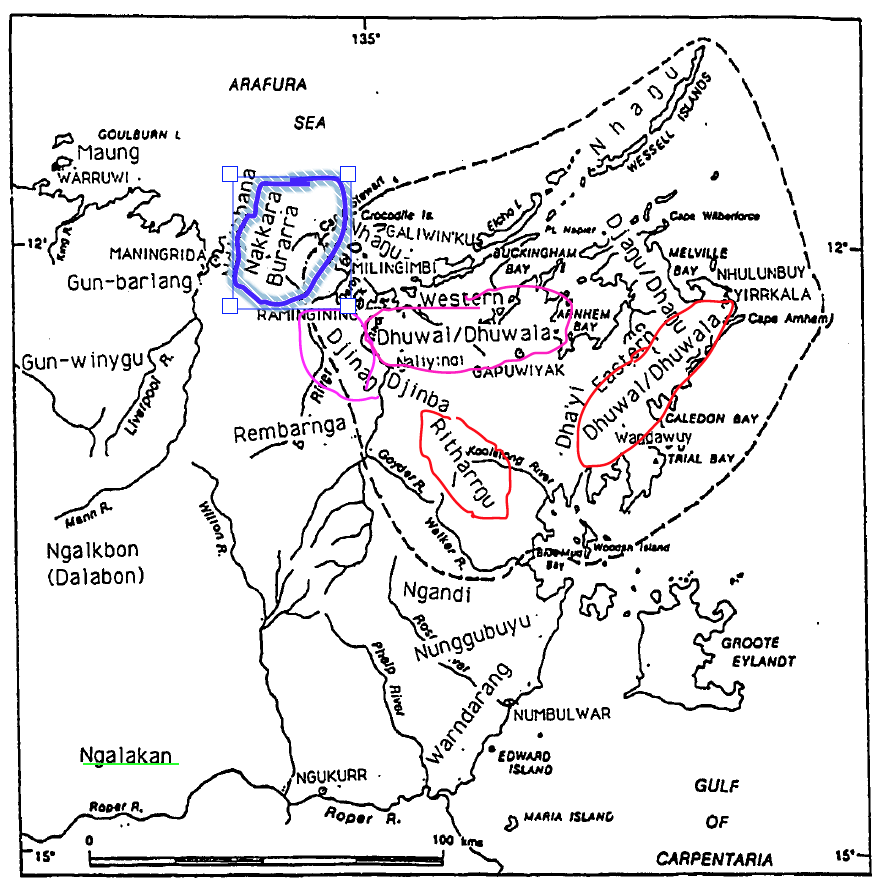
\includegraphics[width=0.75\textwidth]{yolngumatha.png}
\subsection*{Gurr-goni (Arnhem)}
\textbf{Green's work on GURR-GONI }(the language directly to the west of Nakkara in the above map) provides further data on the Arnhem contemporary v. contemporary tense distinction.\footnote{Additionally, I used to work with Bron Eather, who has done work on Nakkara and evidently introduced this contemp v precontemp metalanguage}.
\begin{itemize}
\item \textbf{`today' frame}: contemporary=moment of speech; precontemporary = previous nightfall until `moment before speech'
\item \textbf{`before-today' frame:} contemporary =  several days before today, pre-contemporary = long ago.
\item `between these two poles, there is a large span of time that can be referred to using either tense' (speaker's discretion w/r/t relative recency/distance). The use of the contemporary tense below is an example of
\begin{exe}
\ex\gll gugoni balanda birdibirdi a-garnagirri-\textbf{dji}\\
{\sc iv}-this white\_man recently 3{\sc is}-sit\_down-{\sc \textbf{con}}\\
\glt`White man settled only recently'
\end{exe}
\item \textbf{continuous frame}: Green refers to this as \textit{all time up to and including present}. She claims contemporary tense in this frame refers \textbf{habitual and generic statements} whereas pre-contemporary refers to \textbf{states and events of long ago.}
\end{itemize}
\subsection*{Wangurri (Eastern Yolŋu)}
\begin{enumerate}[1]
\item `neutral' \textit{-Na?$\sim\emptyset$}
\item `pfv' \textit{-(Ka)n(a)?}
\item `hab' \textit{-(Ka)rra}
\item `irr' \textit{-(ŋ)u}
\item `imper' \textit{-Ka}
\end{enumerate}
\begin{itemize}
\item auxiliaries: \textit{bayiŋ} `hab' and \textit{ŋarru} `irr', \textit{gayŋa} `cont'

\item Past readings normally obtain with bare neutral verb form (irr.) as opposed to cooccurring with \textit{gayŋa}.
\item expression of present situation requires an IPFV auxiliary.
\item irrealis marker gives rise to futurate meaning. Where combined with CONT auxiliary, a deontic reading can obtain.
\item {\sc pfv > pst}-shift: the perfective (form 2) only occurs as realis (zero-marked): completeness, boundedness:
\begin{quotation}
Realis implies that the event has happened or is happening. Perfective indicates a boundedness or completeness which is not available to an event that is \textit{happening}. Therefore [the perfective form (2)] is only applicable to an event which has happened. For this reason the perfective in Wangurri also carries the implication of \textit{past event.}
\end{quotation}
\end{itemize}

\subsubsection*{S. Yolŋu -- Dhaŋu/Ritharrŋu}
Heath describes the cognate second form as a regular, absolute `past tense' marker. He pays little attention to its specific semantics claiming there isn't much to report. The small narrative corpus included at the rear of the volume routinely uses the marker to refer to events before present.
\section*{A semantic Change account}

\subsubsection*{Djambarrpuyŋu {\tt[djr]}}
\begin{exe}
\ex\gll yo barpuruɲ ŋarra ŋaɲa nhaa-\textbf{ma}-ɲ\\
yes, yesterday{\sc-prom} 1s 3s{\sc.acc} see-\textbf{1}-{\sc prom}\\
\glt`Yes, I saw him yesterday'
\ex\gll ŋe gaathur ŋarra ŋaɲa nhaa-\textbf{ŋal} goḍarr dhiyal\\
yes, today 1s 3s{\sc.acc} see-\textbf{3} morning {\sc prox-loc}\\
\glt`Yes, I saw him here this morning'
\end{exe}


\subsubsection*{N. Yolŋu} {\tt Wangurri [dhg]}
\begin{exe}
\ex\gll barpuru ŋaya garramaṯpuy \textbf{nhaama} nhaan  barpuru dhal'yun munhaku\\
recently 1s aeroplane see.\textbf{I} 3s recently land-I night\\
\glt`...I \textbf{saw} the aeroplane  yesterday which arrived last night'
\ex\gll ga \textbf{nhaama} ŋanap gayŋa banha ŋunha-l bala gali'-ŋa ga raali-m ŋanapu \textbf{ḏitjun} ga bitjuwayiŋ bayiwitjana-ya ḻiɲgu dhanal banha batjiwarr-murru-m nhana gutjparruwanam\\
and see\textbf{.I} 1p.excl.nom {\sc cont} that there{\sc.loc} {\sc deic} other.side{\sc-loc} and there.d 1p.excl.nom come-\textbf{I} and thus that- because 3p that path 3s.acc \textbf{take{\sc.III-d}}\\
\glt`and \textbf{we could }see there to the other side and we came along that (road) because they had \textbf{taken} him along that road'
\end{exe}

See in (7) above the use of the PFV (inflection 3) in \textit{they had \textbf{taken him along}}. The story is of a group of Indigenous people visiting Israel and recounting their story of retracing the path of Jesus's crucifixion. All events recounted occur before speech time, the reference time is relativised given rise to neutral marking of \textit{nhaama} `see'.
 \end{document}